
% Theory part goes here %

% for numerated formulas
\newcommand{\formula}[3]
{
    \noindent#1\\[0.1cm]
    \begin{equation}\label{#2}
        #3
    \end{equation}
}

% for in-text math formulas
\newcommand{\mth}[1]
{
    \begin{math}
        #1
    \end{math}
}

% for rus letters in indexes
\newcommand{\ruB}[1]
{
    _{\text{#1}}
}

\section{Теоретическая часть}
\subsection{Схема установки}

Схема установки представлена на рисунке 1.

\begin{center}

    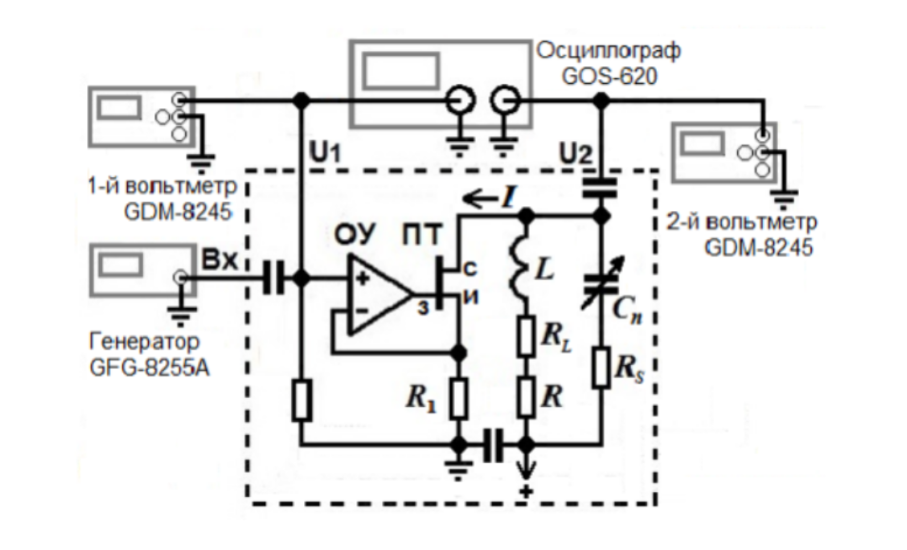
\includegraphics[scale=0.9]{picks/323-scheme.png} \\
    \textit{Рис. 1. Схема установки}

\end{center}

Синусоидальный сигнал от генератора GFG-8255A поступает на вход источника тока, собранного на операционном усилителе ОУ с полевым транзистором ПТ, питание которых осуществляется встроенным блоком-выпрямителем от сети переменного тока 220 вольт. Цепи питания на схеме не показаны, представлен только резистор, переменное напряжение, на котором в используемой схеме равно напряжению на входе «+» операционного усилителя.

Напряжение \mth{E = E_0\cos\left(\omega t + \phi_0\right)} поступает на вход «+» операционного усилителя от генератора через согласующую RC-цепочку. Это же напряжение через разъём «U1» подаётся одновременно на канал 1 осциллографа GOS-620 и вход 1-го цифрового вольтметра GDM-8245. Переменное напряжение на резисторе R1, как отмечалось выше, при этом также равно Е. Напряжение на контуре U, совпадающее с напряжением на конденсаторе, подаётся со знаком «–» через разъём «U2» на канал 2 осциллографа и вход 2-го цифрового вольтметра GDM-8245. Показанные на схеме установки ещё два конденсатора без наименований (помимо входящего в RC-цепочку) играют вспомогательную роль и не влияют на характеристики контура. Символ «->+» отмечает наличие источника питания полевого транзистора. Ток затвора «з» полевого транзистора ничтожно мал, так что токи истока «и» и стока «с» практически совпадают и равны току во внешней цепи контура. Как видно из схемы:

\formula
{}
{CurrentEquation}
{I = \frac{E}{R_1} = I_0\cos\left( \omega t + \phi_0 \right),\qquad I_0 = \frac{E_0}{R1}}

\section{Планируемые исследования}

В работе планируется:

\begin{itemize}
    \item Проведём измерения характеристик контура при разных значениях ёмкости конденсатора. Будем фиксировать резонансные частоты f и напряжения U в контуре при разных C, так же регистрируя входное напряжение E.

    Для расчетов также будут использованы следующие формулы:
    \formula
    {}
    {Zres}
    {Z_{res} = \frac{U}{I_0} = \frac{U}{E/R1}}
    \formula
    {}
    {Rho}
    {\rho = \sqrt{\frac{L}{C}}}
    \formula
    {}
    {Qz}
    {Q = \frac{Z_{res}}{\rho}}
    \formula
    {}
    {Rsumm}
    {R_{\Sigma} = \frac{Z_{res}}{Q^2}}
    \formula
    {}
    {Rsmax}
    {R_{smax} = \frac{\tan(\delta)}{\omega C}}
    \formula
    {}
    {Rl}
    {R_L = R_{smax} - R}

    \item Снимем амплитудно-частотную характеристику контура при ёмкостях C2 и C4. Для этого будем снимать зависимость напряжения в контуре от частоты колебаний.

    \formula
    {Формула для добротности:}
    {Qrlc}
    {Q  =\frac{1}{R}\sqrt{\frac{L}{C}}}

    \item Построим графики АЧХ в координатах\mth {U / U_0 (f / f_0)}. По этим графикам (ширина резонансной кривой на уровне \mth{\frac{1}{\sqrt{2}}}) определим добротность контуров.

    \item Построим ФЧХ для контура с C2 в координатах \mth {x = f / f_0; y = \phi/\pi}. По графику определим добротность контура следующим методом: расстояние между точками по оси x, в которых y меняется от \mth {−\pi/4} до \mth {\pi/4}, равно \mth {1/Q}.

\newpage

    \item Построим векторную диаграмму для токов и напряжений в контуре. Определим значения токов на конденсаторе и на катушке, а также напряжение в контуре, резонансе по формулам:

    \formula
    {}
    {I0}
    {I_0 = \frac{E}{R_1}}
    \formula
    {}
    {Icl}
    {I_C = I_L = QI_0}
    \formula
    {}
    {U}
    {U = Q\rho I_0}
    \formula
    {}
    {PHIc}
    {\phi_C = \frac{\pi}{4} - \frac{R + R_L}{\rho}}
    \formula
    {}
    {PHIl}
    {\phi_L = -\frac{\pi}{2} + \delta}
    \formula
    {}
    {PHIu}
    {\phi_U = \frac{R + R_L}{\rho} + \delta}

\end{itemize}